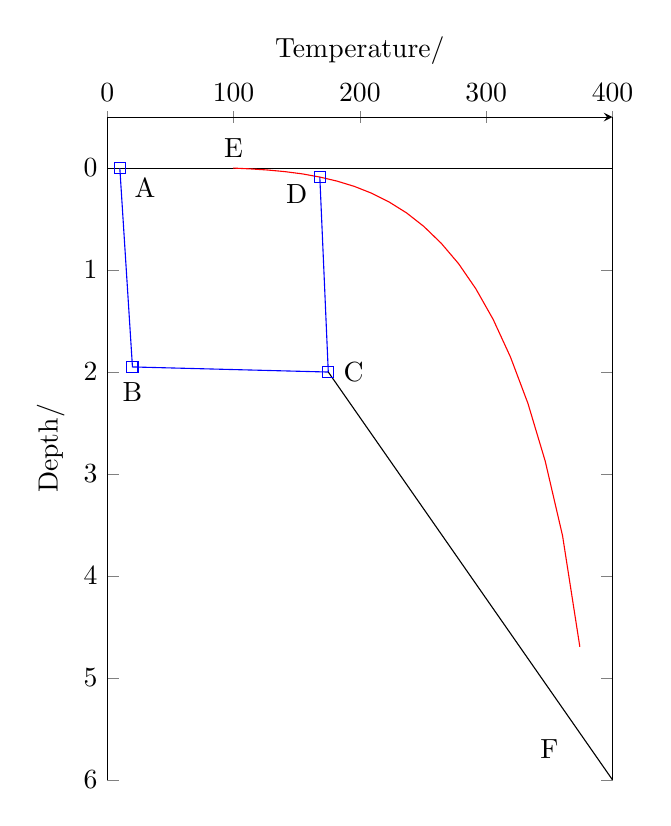
\begin{tikzpicture}[baseline]
    \begin{axis}[y dir = {reverse},
                 xlabel = {Temperature/\unit{\degreeCelsius}},
                 ylabel = {Depth/\unit{\km}},
                 xmin = 0,
                 xmax = 400,
                 ymin = -0.5,
                 ymax = 6,
                 axis x line=top,
                 legend style={at={(0.5,-0.03)}, anchor=north},
                 height=10cm,
                 width=8cm]
        \addplot[color=black]
            coordinates {(0,0)(400,0)};
        
        \addplot[color=red]
            coordinates {(99.6,0.000)  (113.4,0.008)  (127.1,0.019)  (140.8,0.035)  (154.5,0.057)  (168.3,0.088)  (182.0,0.128)  (195.7,0.180)  (209.4,0.247)  (223.2,0.333)  (236.9,0.439)  (250.6,0.572)  (264.3,0.736)  (278.1,0.937)  (291.8,1.184)  (305.5,1.484)  (319.2,1.853)  (333.0,2.307)  (346.7,2.874)  (360.4,3.604)  (374.1,4.694)};
            
        \addplot[color=blue,mark=square]
            coordinates {(10,0)(20,1.95)(175,2)(168.3,0.088)};
        \node at (axis cs:30,0.2) [] {A};
        \node at (axis cs:20,2.2) [] {B};
        \node at (axis cs:195,2) [] {C};
        \node at (axis cs:150,0.25) [] {D};
        \node at (axis cs:100,-0.2) [] {E};
        
        \addplot[color=black]
            coordinates {(400,6)(175,2)};
        \node at (axis cs:350,5.7) [] {F};
            
    \end{axis}
\end{tikzpicture}%
~%
%
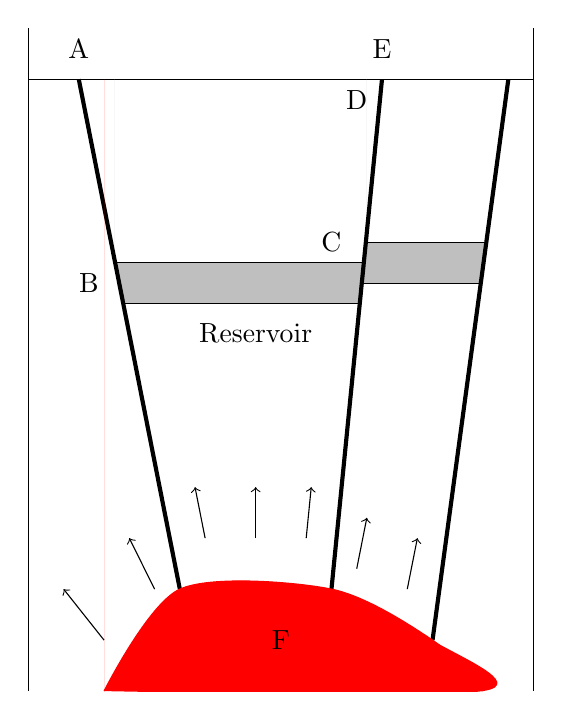
\begin{tikzpicture}[baseline]
    \begin{axis}[y dir = {reverse},
                 xmin = 0,
                 xmax = 100,
                 ymin = -0.5,
                 ymax = 6,
                 axis x line=top,
                 axis x line=none,
                 legend style={at={(0.03,0.03)}, anchor=south west},
                  height=10cm,
                 width=8cm,
                 ticks=none]
        % add the surface
        \addplot[color=black]
            coordinates {(0,0)(400,0)};
            
        % adding the reservoir
        \addplot[fill=lightgray,draw=none] coordinates {(17,1.8) (18.5,2.2) (65.5,2.2) (66.5,1.8) (17, 1.8)} \closedcycle;
        \addplot[color=black]
            coordinates {(17,1.8)(66,1.8)};
        \addplot[color=black]
            coordinates {(19,2.2) (66,2.2)};
        \node at (axis cs:45,2.3) [anchor=north] {Reservoir};

        \addplot[fill=lightgray,draw=none] coordinates {(67,1.6) (66,2.0) (89.5,2.0) (91,1.6) (67, 1.6)} \closedcycle;
        \addplot[color=black]
            coordinates {(67,1.6)(91,1.6)};
        \addplot[color=black]
            coordinates {(66,2.0) (90,2.0)};

        % adding the faults
        \addplot[color=black, line width=1.5pt]
            coordinates {(10,0)(30,5)};
        \addplot[color=black, line width=1.5pt]
            coordinates {(60,5) (70,0)};
        \addplot[color=black, line width=1.5pt]
            coordinates {(80,5.5) (95,0)};

        % adding the heat source
        \addplot[fill=red,draw=none, smooth] coordinates {(15,6) (30,5) (60,5) (80,5.5) (90, 6) (15, 6)} \closedcycle;
        \addplot[smooth,color=red]
            coordinates {(15,6)(30,5)(60,5)(80,5.5)(90,6)};
        \node at (axis cs:50,5.5) [color=black] {F};

        % adding the fluid pathway
        \node at (axis cs:10,-0.3) [] {A};
        \node at (axis cs:12,2) [] {B};
        \node at (axis cs:60,1.6) [] {C};
        \node at (axis cs:65,0.2) [] {D};
        \node at (axis cs:70,-0.3) [] {E};

        % add conduction arrows
        \draw[->](axis cs:15,5.5)--(axis cs:7,5);
        \draw[->](axis cs:25,5)--(axis cs:20,4.5);
        \draw[->](axis cs:35,4.5)--(axis cs:33,4);
        \draw[->](axis cs:45,4.5)--(axis cs:45,4);
        \draw[->](axis cs:55,4.5)--(axis cs:56,4);
        \draw[->](axis cs:65,4.8)--(axis cs:67,4.3);
        \draw[->](axis cs:75,5)--(axis cs:77,4.5);
        
    \end{axis}
\end{tikzpicture}